Una forma de resolver este problema es obtener una relación de recurrencia para un $n$ dado en términos de m. Por ejemplo, si $n=2$, obtenemos la relación de recurrencia:

$$f_{m} = f_{m-1} + f_{m-2}$$

Y si $n=3$, obtenemos la relación de recurrencia.

$$f_{m} = 4f_{m-1} - f_{m-2}$$

Que sale del siguiente análisis. Sea $f_n$ el número de formas de colocar fichas de dominó en una cuadrícula de $2 \times n$.

Considere el primer cuadrado de la cuadrícula (el cuadrado más a la izquierda de la primera fila),

\begin{itemize}
	\item Podrías colocar una ficha de dominó verticalmente sobre eso, por lo que hay $f_{n-1}$ formas de 
	colocar en mosaico el resto de la cuadrícula.
	\item O puedes colocar el dominó horizontalmente sobre él, por lo que debes colocar otro dominó 
	horizontalmente debajo y hay $f_{n-2}$ formas de colocar en mosaico el resto de la cuadrícula.
\end{itemize}

Así que tenemos $f{n}=f{n-1}+f{n-2}$. Necesitamos calcular $f_1$ y $f_2$ y luego podemos calcular $f_n$ para cualquier número natural.

No es difícil ver que $f_1=1$ y $f_2=2$.

Para la cuadrícula de $3$ por $2n$, sea $f_n$ el número de formas de mosaico de la cuadrícula de $3$ por $2n$ con fichas de dominó y $g_n$ sea el número de formas de mosaico de una cuadrícula de $3$ por $2n+1$ a la que le falta su primer cuadrado.

Utilice el método anterior para demostrar que,

$$f_n=2g_{n-1}+f_{n-1}$$

y

$$g_n=f_n+g_{n-1}$$

Ahora deberías resolver estas ecuaciones para ver que:

$$f_{m} = 4f_{m-1} - f_{m-2}$$

Y nuevamente también debes calcular $f_1$ y $f_2$.

Pero obtener la relación de recurrencia se vuelve más difícil a medida que $n$ aumenta. Por lo tanto, abordaremos este problema de una manera diferente. Definamos el perfil de alguna columna como un entero binario de $n$ bits que proporciona información sobre la ocupación de los bloques en esa columna, es decir, si el i-ésimo bit es igual a 1, entonces el i-ésimo bloque de esa columna está ocupado por alguna ficha de dominó y si es igual a 0 entonces no está ocupado. Definamos nuestro estado DP como $dp[i][p]$ (indexación basada en 1), que es igual al número de formas de llenar las primeras i columnas completamente con fichas de dominó (sin dejar ningún bloque vacío). Aquí $p$ es el perfil de la (i+1)ésima columna obtenida después de llenar las primeras $i$ columnas. Tenga en cuenta que la (i+1)ésima columna no debe contener una ficha de dominó completa ya que nuestra intención es usar fichas de dominó para llenar la primera $i$ columnas. Aquí hay un ejemplo.

% TODO: \usepackage{graphicx} required
\begin{figure}[!h]
	\centering
	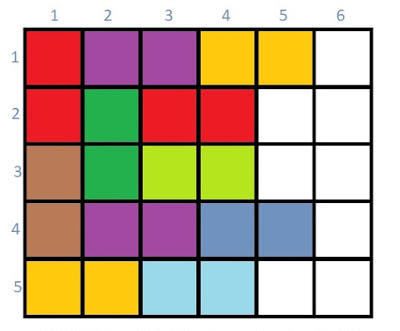
\includegraphics[width=0.5\linewidth]{img/counting_tiling_1}
	\caption{Relleno válido de las primeras 4 columnas dejando la quinta columna con el perfil 9, es decir, 01001}
	\label{fig:countingtiling1}
\end{figure}

\begin{figure}[!h]
	\centering
	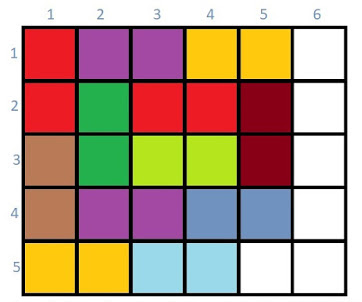
\includegraphics[width=0.5\linewidth]{img/counting_tiling_2}
	\caption{Relleno no válido que no se puede contar en dp[4][5] ya que el dominó marrón no se utiliza para rellenar ninguna de las primeras cuatro columnas. Nota: 15 representa 01111, es decir, el perfil de la quinta columna}
	\label{fig:countingtiling2}
\end{figure}

Pero ¿cómo obtenemos la relación entre los estados? Una forma es obtener el valor de \(dp[i][p]\) de \(dp[i-1][q]\) expresando el primero como la suma de todos \(dp[i-1] [q]\) para lo cual existe un relleno de la \((i)\)ésima columna con fichas de dominó, dejando la \(i+1\)ésima columna con el perfil \(p\). La complejidad del tiempo para calcular \(dp[i][p]\) es igual a \(O(2^n)\). Como hay \(m \times 2^n\) estados, la complejidad del tiempo total se vuelve igual a \(O(m \times 2^{2n})\).


Pero obtendríamos un veredicto de TLE para el algoritmo anterior. Para evitar esto, en lugar de encontrar todos los perfiles posibles \(q\) tales que \(dp[i-1][q]\) pueda producir \(dp[i][p]\), para un perfil determinado \( q\) encontramos todos los perfiles posibles \(p\) tales que \(dp[i-1][q]\) pueda producir \(dp[i][p]\) y sumamos el valor de \(dp[ i-1][q]\) a \(dp[i][p]\). Esto significa que verificamos todas las formas posibles de llenar la \(i\)ésima columna que tiene el perfil \(q\). Para hacer esto, analicemos la \(i\)ésima columna desde el \(1\)er bloque de la columna hasta el \(n\)ésimo bloque de la columna.

Si el \(j\)ésimo bloque ya está ocupado por alguna ficha de dominó, entonces no hagas nada.
De lo contrario, este bloque se puede completar como máximo de dos maneras, como se detalla a continuación.

\begin{enumerate}
	\item Coloque una ficha de dominó en los bloques \((i,j)\) y \((i+1,j)\) y márquelos como ocupados.
	\item Coloque una ficha de dominó en los bloques \((i,j)\) y \((i,j+1)\) y márquelos como ocupados si el bloque (\(j+1)\) existe y está desocupado.
\end{enumerate}

Cada permutación que llena la columna actual produce un perfil único \(p\) que representa la \((i+1)\)ésima columna. Entonces agregamos \(dp[i][q]\) a \(dp[i+1][p]\) donde \(q\) es el perfil de la \(i\)ésima columna antes del llenado.

Ahora, observe que para \(i = 0\), llenar las primeras \(0\) columnas completamente y tener el perfil \(p\) para la \(1\)st columna es posible si \(p = 0\). Esto implica que \(dp[0][p]\) es igual a \(1\) para \(p = 0\) e igual a \(0\) para todo \(p \neq 0\).

Dado que necesitamos llenar todas las \(m\) columnas con el perfil para la \((m+1)\)ésima columna igual a 0 (ya que no existe ninguna \((m+1)\)ésima columna), el requerido la respuesta es igual a \(dp[m][0]\).